\setcounter{chapter}{11}

\chapter{曲线积分与曲面积分}

\section{曲线积分}

\subsection{对弧长的曲线积分}

\subsubsection{1、平面曲线的长度}

{\bf 例:}求以下曲线的长度
\begin{enumerate}[(1)]
  \setlength{\itemindent}{1cm}
  \item $y=x^2,\;(0\leq x\leq 3)$
  \item $x^2+y^2=2x$
  \item $\rho=\cos\theta,\;(\theta\in[0,2\pi])$
\end{enumerate}

\begin{description}
\item[{\bf 弧微分:}] 弧长的微元
	$$\d s=\sqrt{(\d x)^2+(\d y)^2}$$
	$$\d s=\sqrt{1+(y'_x)^2}\d x=\sqrt{(x'_t)^2+(y'_t)^2}\d t
	=\sqrt{(\rho'_{\theta})^2+\rho^2}\d\theta$$
\item[{\bf 曲线长度:}] 弧长微元的总和
	$$s=\dint_L\d s$$
\end{description}

\subsubsection{2、空间曲线的长度}

{\bf 例:}计算圆柱螺旋线$x=\cos t,y=\sin t,z=t,(0\leq t\leq 2\pi)$的长度。

设$L:\bm{r}(t)=(x(t),y(t),z(t)),\;(a\leq t\leq b)$, 则
$${\d s=\sqrt{(\d x)^2+(\d y)^2+(\d z)^2}
=\sqrt{(x'_t)^2+(y'_t)^2+(z'_t)^2}\d t} =|\bm{r}'(t)|\d t$$
从而曲线长度
$${s=\dint_L\d s =\dint_a^b\sqrt{(x'_t)^2+(y'_t)^2+(z'_t)^2}\d t
 =\dint_a^b|\bm{r}'(t)|\d t}$$

\subsubsection{3、对弧长的曲线积分}

$$\dint_Lf(x,y,z)\d s$$

{\bf 例:}已知空间曲线$L:\bm{r}(t)=(x(t),y(t),z(t)),\;(a\leq t\leq b)$,其上
的线密度为$\mu(x,y,z)$,求:
\begin{enumerate}
  \item 曲线的质量
  \item 曲线的质心
  \item 关于$z$轴的转动惯量
  \item 对位于$(a,b,c)$质量为$m$的质点的万有引力
\end{enumerate}

\subsubsection{4、性质}

$${I=\dint_Lf(x,y,z)\d s=\dint_a^bf(x,y,z)|\bm{r}'(t)|\d t}$$

{\bf 约定:}计算对弧长的曲线积分时,应确保积分上限总是大于积分下限的!

\begin{enumerate}[(1)]
  \setlength{\itemindent}{1cm}
  \item {\bf 线性性} 
  \item {\bf 无向性}
  $$\dint_Lf(x,y,z)\d s=\dint_{L^-}f(x,y,z)\d s$$
  \item {\bf 路径可加性}
  $$\dint_{L_1+L_2}f(x,y,z)\d s=\left(\dint_{L_1}+\dint_{
  L_2}\right)f(x,y,z)\d s$$
\end{enumerate}

{\bf 注:}定积分可以视为对$x$轴的弧长的曲线积分!

\subsubsection{5、计算}

{\bf 例:}设有点$A(1,1,0)$和$B(1,1,1)$,$L$为线段$OA,AB$和$BO$组成的封闭曲线,
方向为$O\to A\to B\to O$,计算曲线积分
$$\oint_L(x+y+z)\d s.$$

{\bf 计算步骤:}曲线(分段)参数化$\to$定限$\to$积分

\subsection{对坐标的曲线积分}

\subsubsection{1、概念}

{\bf 例:}已知某质点$M$在{\bf 引力场}
$$\bm{F}(x,y,z)=(P(x,y,z),Q(x,y,z),R(x,y,z))$$
中沿曲线$L:\bm{r}(t)=(x(t),y(t),z(t)),(a\leq t\leq b)$
运动,求引力对其做的功。

$${W=\dint_L\bm{F}\d\bm{s}=\dint_LP\d x+\dint_LQ\d y+\dint_LR\d z}$$

其中,若$L$为封闭曲线,则可记为:
$$W=\oint_LP\d x+Q\d y+R\d z$$

\subsubsection{2、性质}

\begin{enumerate}[(1)]
  \setlength{\itemindent}{1cm}
  \item {\bf 有向性:}
  $$\dint_LP\d x+Q\d y+R\d z=-\dint_{L^-}P\d x+Q\d y+R\d z$$
  \item {\bf 路径可加性:} 设$L=\bigcup_{k=1}^nL_k$, 且$L$与$L_k(k=1,2,\ldots,n)$
  方向均一致, 则
  $$\dint_LP\d x+Q\d y+R\d z=\sum\limits_{k=1}^n\dint_{L_k}P\d x+Q\d y+R\d z$$
\end{enumerate}

\subsubsection{3、计算}

{\bf 例:}设有点$A(1,1,0)$和$B(1,1,1)$,$L$为线段$OA,AB$和$BO$组成的封闭曲线,
方向为$O\to A\to B\to O$,分别计算曲线积分
$$\oint_L(x+y+z)\d s\quad\mbox{和}\quad\oint_Lx\d x+y\d y+z\d z.$$

{\bf 计算步骤:}曲线(分段)参数化$\to$定限$\to$积分

\subsection{两类曲线积分的关系}

设$L:\bm{r}(t)=(x(t),y(t),z(t)),\;(a\leq t\leq b)$, 其单位切向量
$$\bm{T}=\df{\bm{r}'(t)}{|\bm{r}'(t)|}$$
 则$\bm{T}$与$L$同向,
$${\dint_L\bm{F}\cdot \d\bm{s}=\dint_L\bm{F}\cdot\bm{T}\d s}$$
% 	=\dint_L\bm{F}\cdot\bm{r}'(t)\d t}$$
即:{对坐标的曲线积分总可以化为对弧长的曲线积分}
 
{\bf 例:}计算曲线积分$\dint_Lxy\d x$,其中积分曲线$L$分别为:
\begin{enumerate}[(1)]
  \setlength{\itemindent}{1cm}
  \item 由原点沿$y=x^3$至$A(1,1)$;
  \item 由原点沿$y^2=x$至$A(1,1)$。
\end{enumerate}

{\bf 例:}计算曲线积分$\dint_Ly\d x-x\d y$,其中积分曲线$L$分别为:
\begin{enumerate}[(1)]
  \setlength{\itemindent}{1cm}
  \item 由$A(0,-1)$沿右半单位圆至$B(0,1)$;
  \item 由$A(0,-1)$沿左半单位圆至$B(0,1)$;
  \item 由$A(0,-1)$沿单位圆逆时针方向至$A(0,-1)$。
\end{enumerate}

\subsection{曲线积分的应用}

\begin{enumerate}
  \item {\bf 对弧长的曲线积分:}
  \begin{itemize}
    \item 曲线的长度、质量
    \item 曲线的质心、转动惯量
    \item 曲线对质点的引力
  \end{itemize}
  \item {\bf 对坐标的曲线积分:}
  \begin{itemize}
    \item 变力沿曲线做功
    \item {向量场中的环量和流量}
  \end{itemize}
\end{enumerate}

\subsubsection{流量与环量}

考虑平面区域内$D$内的向量场
$$\bm{v}=(P(x,y),Q(x,y)),\;(x,y)\in D.$$
$L:\bm{r}=\bm{r}(t)$为$D$内简单光滑闭曲线,取逆时针方向。
$\bm{T},\bm{n}$分别为$L$的单位切向量和单位法向量。
\begin{itemize}
  \item {\bf 流量:}$\ds\oint_L\bm{v}\cdot\bm{n}\d s$
  {\;—“向量场穿过$L$的总量”}
  \item {\bf 环量:}$\ds\oint_L\bm{v}\cdot\bm{T}\d s$
  {\;—“向量场环绕$L$的总量”}
\end{itemize}

\begin{center}
	\resizebox{!}{5cm}{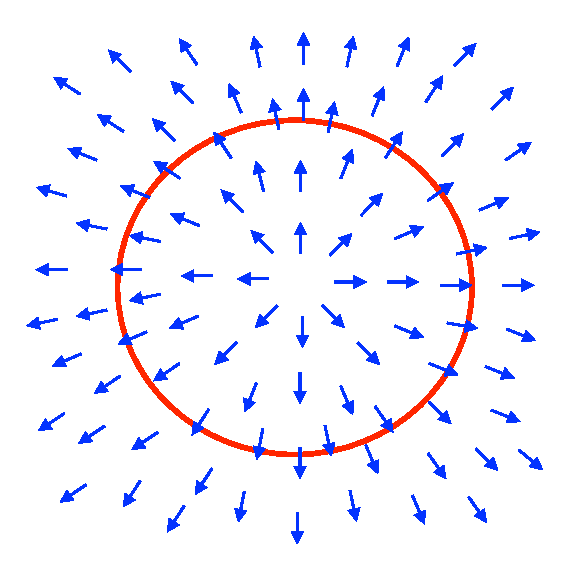
\includegraphics{./images/ch12/flow.pdf}}\hspace{2cm}
	\resizebox{!}{5cm}{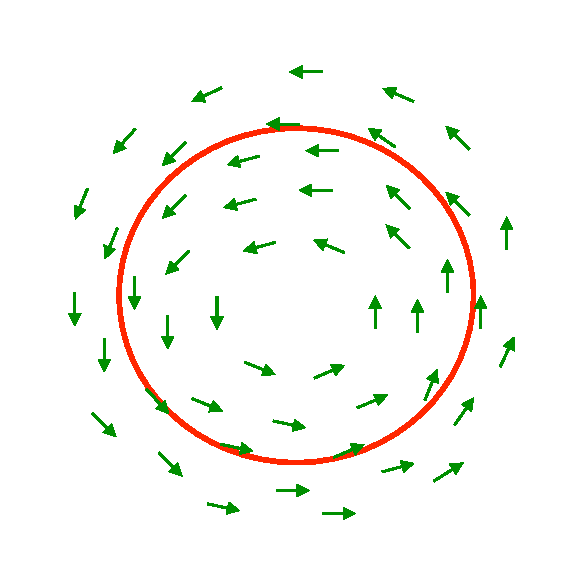
\includegraphics{./images/ch12/rotate.pdf}}
	
	{\bf 流量:}${\ds\oint_L\bm{v}\cdot\bm{n}\d s}$\hspace{4cm}
	{\bf 环量:}${\ds\oint_L\bm{v}\cdot\bm{T}\d s}$
\end{center}

{\bf 例:}分别计算向量场
$$\bm{v}_1=(x,y)\quad\mbox{和}\quad \bm{v}_2=(-y,x)$$
沿单位圆逆时针方向的流量和环量。

\section{Green公式与保守场}

\subsection{Green公式}

{\bf 定理12.2.1-3:}$$\oint_LP(x,y)\d x+Q(x,y)\d y=\iint_D\left(
\df{\p Q}{\p x}-\df{\p P}{\p y}\right)\d\sigma$$

\begin{itemize}
  \item $D$$xOy$平面内的有界闭区域
  \item $L=\p D$:分段光滑曲线,按{\it “左侧法则”}取正向
  \item $P(x,y),Q(x,y)$在$D$内有连续偏导数
\end{itemize}

{\bf 例:}沿单位圆的逆时针方向计算以下曲线积分
$$\oint_Lx\d x+y\d y,\hspace{3em}\oint_Ly\d x+x\d y$$

{\bf 说明:}
\begin{enumerate}[(1)]
  \setlength{\itemindent}{1cm}
  \item {\bf 左侧法则:}积分区域始终位于曲线方向的左侧;
  \item 区域$D$必须有界;
  \item $D$的边界可以包含平行于$x$轴和$y$轴的直线;
  \item $D$可以是简单闭区域、单连通域和多连通域;
\end{enumerate}

{\bf 例:}计算椭圆$\df{x^2}{a^2}+\df{y^2}{b^2}\leq 1\,(a>0,b>0)$的面积。

$$\oint_L x\d y-y\d x=2\iint_D\d\sigma$$

{\bf 例:}设有流速场
$$\bm{v}(x,y)=\left(\df{x}{x^2+y^2},
\df{y}{x^2+y^2}\right),\;(x^2+y^2\ne 0),$$
求其通过以下闭曲线(均取逆时针方向)的流量:
\begin{enumerate}
  \setlength{\itemindent}{1cm}
  \item $L_1$:不经过原点且不包含原点的任一光滑闭曲线;
  \item $L_2$:$x^2+y^2=R^2$
  \item $L_3$:$\df{x^2}{a^2}+\df{y^2}{b^2}=1\,(a>0,b>0)$
\end{enumerate}

\subsection{向量场与Green公式}

\subsubsection{散度与无源场}

已知流速场
$$\bm{v}=(P(x,y),Q(x,y)),\;(x,y)\in D,$$
满足Green公式条件 ,则
\begin{enumerate}
  \item {\bf 散度:}${\mathrm{div}\,\bm v=\df{\p P}{\p x}+\df{\p Q}{\p
  y}}$ 
  $$\oint_L\bm{v}\cdot\bm{n}\d
  s=\iint_D\mathrm{div}\,\bm{v}\,\d\sigma$$
  \item {\bf 无源场:}${\mathrm{div}\,\bm{v}=0}$
\end{enumerate}

\subsubsection{无旋场}

已知流速场
$$\bm{v}=(P(x,y),Q(x,y)),\;(x,y)\in D,$$
满足Green公式条件 ,则
$$\oint_L\bm{v}\cdot\bm{T}\d s=\iint_D\left(
\df{\p Q}{\p x}-\df{\p P}{\p y}\right)\d\sigma $$
\begin{enumerate}
  \addtocounter{enumi}{2}
  \item {\bf 无旋场:}${\df{\p Q}{\p x}-\df{\p P}{\p y}=0}$
\end{enumerate}

{\bf 定理:}
\begin{enumerate}[(1)]
  \setlength{\itemindent}{1cm}
  \item 区域$D$内的向量场为无源场,则通过$\p D$的流量为$0$
  \item 区域$D$内的向量场为无旋场,则沿$\p D$的环量为$0$
\end{enumerate}

\subsection{保守场与积分路径无关性}

设区域$D$内有向量场
$\bm{F}(x,y)=(P(x,y),Q(x,y))$,
在$D$内任取两点$A,B$,若由$A$到$B$沿任意路径所做的功都一样,
也即积分
$$\dint_{L_{AB}}P\d x+Q\d y$$
的值是与积分路径无关的,
则称$\bm{F}(x,y)$为区域$D$内的一个保守场

{\bf 定理12.2.4}(保守场的判定)$\bm{F}(x,y)=(P(x,y),Q(x,y))$为单连通域$D$内的向量场,
$P,Q$具有一阶连续偏导数,则以下条件等价:
\begin{enumerate}[(1)]
  \setlength{\itemindent}{1cm}
  \item $\bm{F}$是$D$内的保守场;
  \item $\bm{F}$是$D$内的无旋场;
  \item 存在$u(x,y)$,使得
  $$\d u(x,y)=P(x,y)\d x+Q(x,y)\d y,\;(x,y)\in D$$
\end{enumerate}

\subsection{原函数与全微分}

$\bm{F}=(P,Q)$是$D$内的保守场,则存在$u(x,y)$,使得
$$\d u(x,y)=P(x,y)\d x+Q(x,y)\d y,\;(x,y)\in D$$
 $u(x,y)$称为: 
\begin{itemize}
  \item {\bf 微分式$P\d x+Q\d y$的原函数} 
  \item {\bf 向量场$\bm{F}$的势函数} 
\end{itemize}
\bigskip
$${\dint_{L_{AB}}P\d x+Q\d y=u(x,y)|_A^B} $$
{\bf 注:}$u(x,y)$不唯一!

{\bf 原函数的计算——折线法:}

$\bm{F}=(P,Q)$是$D$内的保守场,求其势函数$u(x,y)$

\begin{enumerate}[Step1]
  \setlength{\itemindent}{1cm}
  \item 任取$A(x_0,y_0),\,B(x,y)\in D$ 
  \item 取折线
  $${L:\,A(x_0,y_0)\to C(x,y_0)\to B(x,y)} $$
  \item 计算积分
  \begin{eqnarray*}
  	u(x,y)&=&\dint_LP(x,y)\d x+Q(x,y)\d y \\
  	&=&{\dint_{x_0}^xP(x,y_0)\d x+\dint_{y_0}^yQ(x,y)\d y}
  \end{eqnarray*}
\end{enumerate}

{\bf 例:}验证向量场
$$\bm{F}=(4x^3y^3-3y^2+5,3x^4y^2-6xy-4)$$
为$xOy$平面上的保守场,并求$\bm{F}$的势函数。利用势函数计算
$\bm{F}$沿以$(0,1)$为起点,$(1,2)$为终点的路径所做的功。

{\bf 习题12.2-6:}求下列全微分的原函数
\begin{enumerate}[(1)]
  \setlength{\itemindent}{1cm}
  \item $(x^2+2xy-y^2)\d x+(x^2-2xy-y^2)\d y$
  \item $e^x[e^y(x-y+2)+y]\d x+e^x[e^y(x-y)+1]\d y$
  \item $f(\sqrt{x^2+y^2})x\d x+f(\sqrt{x^2+y^2})y\d y$
\end{enumerate}

{\bf 习题12.2-17:}利用全微分法计算曲线积分
\begin{enumerate}[(1)]
  \setlength{\itemindent}{1cm}
  \item $\dint_{(1,1,1)}^{(2,3,-4)}x\d x+y^2\d y-z\d z$
  \item $\dint_{(1,1,1)}^{2,3,-4}(x+y+z)^3(\d x+\d y+\d z)$
\end{enumerate}

{\bf 定义:}若存在$u(x,y)$,满足:
$$\d u(x,y)=P(x,y)\d x+Q(x,y)\d y,$$
则称{\it $P(x,y)\d x+Q(x,y)\d y=0$为全微分方程}

{\bf 注:}$P(x,y)\d x+Q(x,y)\d y=0$为全微分方程当且仅当
$$\df{\p P}{\p y}=\df{\p Q}{\p x}$$

{\bf 例:}求微分方程
$$(3x^2+6xy^2)\d x+(6x^2y+4y^3)\d y=0$$
的通解。

{\bf 积分因子法求解微分方程:}

{\bf 例:}求解微分方程:$x\d y-y\d x=0$。

通过两边同时乘以特定的函数({\it 积分因子}),可以使原方程化为全微分方程:
$${\df 1{y^2}}(x\d y-y\d x) =-\d\left(\df xy\right)
=0,\quad {\df{1}{x^2+y^2}}(x\d y-y\d x) =-\d\arctan\df xy=0$$

\section{曲面积分}

\subsection{对面积的曲面积分}

{\bf 如何求空间曲面$\Sigma:\,z=f(x,y),\,(x,y)\in D$的面积?}

{\bf 例:}求空间曲面$\Sigma:z=x,(x,y)\in D$的面积,其中:
\begin{enumerate}[(1)]
  \setlength{\itemindent}{1cm}
  \item $D:\,0\leq x\leq 1,\,0\leq y\leq 1$
  \item $D:\,x^2+y^2\leq 1$
\end{enumerate}

\begin{center}
	\resizebox{!}{4cm}{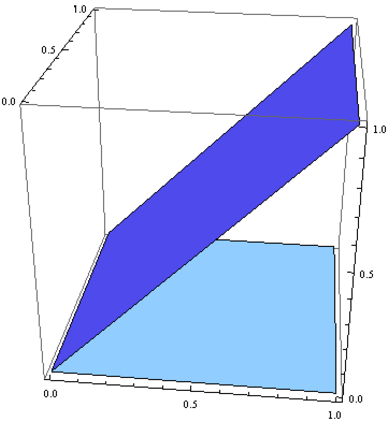
\includegraphics{./images/ch12/ssquare.pdf}}
	\hspace{3cm}
	\resizebox{!}{4cm}{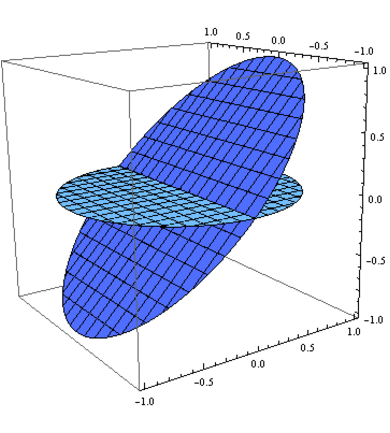
\includegraphics{./images/ch12/scircle.pdf}}
\end{center}

{\bf 例:}推导球表面积公式。

$${S=\iint_{\Sigma}\d S
=\iint_D\sqrt{1+(f\,'_x)^2+(f\,'_y)^2}\d\sigma}$$

{\bf 例:}设空间曲面$\Sigma:\,z=f(x,y),\,(x,y)\in D$的面密度函数为
$f(x,y,z)$,求其质量。

$${M=\iint_{\Sigma}f(x,y,z)\d S}$$

{\bf 习题12.3-16:}证明:曲线$y=f(x),x\in[a,b]$绕$y$轴旋转所得
曲面侧面积$S=2\pi\dint_Lf(x)\d s$,且
$$S=2\pi\dint_a^bf(x)\sqrt{1+[f'(x)]^2}\d x$$

\begin{itemize}
  \item {\bf 应用:} 质心、 转动惯量、 万有引力 
  \item {\bf 性质:} 线性性、 曲面的可加性
\end{itemize}

{\bf 例:}计算曲面积分
$$I=\oiint_{\Sigma}x^2\d S,$$
其中$\Sigma$为$x+y+z=1$和坐标平面所围立体的表面。

{\bf 步骤:}选择投影方向 $\to$写出面积微元 $\to$计算二重积分

{\bf 例:}计算曲面积分
$$\iint_{\Sigma}z\d S,$$
其中$\Sigma$为柱面$x^2+y^2=1$夹在平面$z=0$和$z=1+x$之间
的部分。

{\bf 例:}设函数$y=f(x)$在区间$[a,b]$上连续可导、非负,证明其
绕$x$轴旋转所得曲面面积为
$$S=2\pi\dint_a^bf(x)\sqrt{1+(f\,'_x)^2}\d x$$

\subsection{对坐标的曲面积分}

{\bf 例:}已知曲面$\Sigma:\,z=f(x,y),\,(x,y)\in D$和流速场
$$\bm{v}(x,y,z)=(P(x,y,z),Q(x,y,z),R(x,y,z)),$$
求经过该曲面的流量。

{\bf 约定:}沿给定法方向流过$\Sigma$的流量为正,反之为负

\begin{enumerate}
  \item {\bf 双侧曲面:}
  \begin{itemize}
    \item {\bf 封闭曲面:外侧为正,内侧为负}
    \item 开放曲面:任取一侧为正,一侧为负
  \end{itemize}
  \item {\bf 单侧曲面:}无方向
\end{enumerate}
\begin{center}
	\resizebox{!}{2.5cm}{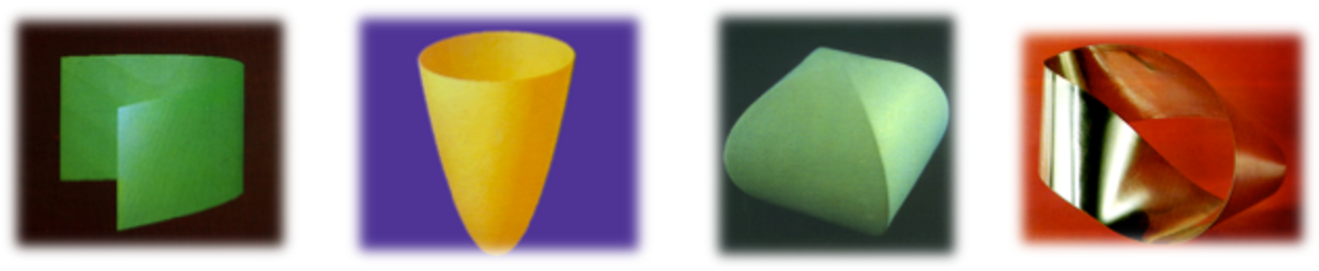
\includegraphics{./images/ch12/ss.pdf}}
\end{center}

$${\Phi=\iint_{\Sigma}\bm{v}\cdot\bm{n}\d S}$$
其中$\bm{n}$沿曲面正向的单位法向量。

注意到
$$\bm{n}\d S=(\d\sigma_{yz},\d\sigma_{zx},\d\sigma_{xy})
=(\d y\d z,\d z\d x,\d x\d y),$$
故
$${\Phi=\iint_{\Sigma}P(x,y,z)\d y\d z
+Q(x,y,z)\d z\d x+R(x,y,z)\d x\d y}$$

{\bf 例:}已知曲面$\Sigma:\,z=f(x,y),\,(x,y)\in D$,计算
$$I=\iint_{\Sigma}R(x,y,z)\d x\d y$$

\begin{enumerate}[(1)]
  \setlength{\itemindent}{1cm}
  \item {\bf 曲面的参数方程:} $x=x,y=y,z=z(x,y)$ 
  \item {\bf 判断曲面方向:}若曲面正向与$z$轴成锐角,取正号;反之为负 
\end{enumerate}
$${I=\pm\iint_DR(x,y,z(x,y))\d x\d y}$$

{\bf 例:}计算曲面积分
$$I=\oiint_{\Sigma}xyz\d x\d y,$$
其中$\Sigma$由四分之一单位球面($x\geq 0,y\geq 0$)和
$x=0,y=0$共同组成。

\subsection{曲面积分的应用}

\begin{enumerate}
  \item {\bf 对面积的曲面积分:} 
  \begin{itemize}
    \item 曲面的质量 
    \item 质心 
    \item 转动惯量 
    \item 万有引力 
  \end{itemize}
  \item {\bf 对坐标的曲面积分:} 
  \begin{itemize}
    \item 流量
  \end{itemize}
\end{enumerate}

{\bf 例:}设半球壳$z=\sqrt{R^2-x^2-y^2}$的密度为常数$\mu$,求:
\begin{enumerate}[(1)]
  \setlength{\itemindent}{1cm}
  \item 半球壳的质心;
  \item 半球壳关于$z$轴的转动惯量。
\end{enumerate}

{\bf 例:}将半径为$R$的球体置于水中,顶部与水面相切,求球的上半部分所受水的压力。

{\bf 例:}已知流速场$\bm{v}=(0,yz,z^2)$,求穿过柱面
$y^2+z^2=1(z\geq 0)$被$x=0$和$x=1$所夹部分的流量,
取曲面上侧为其正向。

\section{Gauss公式和Stokes公式}


{\bf Green公式}
$$\oint_LP(x,y)\d x+Q(x,y)\d y=\iint_D\left(
\df{\p Q}{\p x}-\df{\p P}{\p y}\right)\d\sigma $$

\begin{itemize}
  \item {$D$:}$xOy$平面内的{\it 有界闭区域}
  \item {$L=\p D$:}分段光滑曲线,按{\it “左侧法则”}取正向
  \item {$P(x,y),Q(x,y)$:}在$D$内有连续偏导数
\end{itemize}

\subsection{Green公式流量形式的三维推广——Gauss公式}

{\bf Green公式:}平面向量场$\bm{v}$,平面区域$D$,$L=\p D$
$${\oint_L\bm{v}\cdot\bm{n}\d s=\iint_D\mathrm{div}\,\bm{v}\d\sigma}$$

{\bf 推广:}空间向量场$\bm{v}$, 空间区域$\Omega$, $\Sigma=\p\Omega$
$${\oiint_{\Sigma}\bm{v}\cdot\bm{n}\d
s=\iiint_{\Omega}\mathrm{div}\,\bm{v}\d\sigma}$$

{\bf 定理12.4.1}(Gauss公式)
$$\oiint_{\Sigma}P\d y\d z+Q\d z\d x+R\d x\d y=\iiint_{\Omega}
\left(\df{\p P}{\p x}+\df{\p Q}{\p y}+\df{\p R}{\p z}\right)\d V$$

\begin{itemize}
  \item {$\Omega$:}空间{\it 有界闭区域}
  \item {$\Sigma=\p\Omega$:}分片光滑曲面,取{\it “外侧”}为正向
  \item {$P(x,y,z),Q(x,y,z),R(x,y,z)$:}在$\Omega$内偏导连续
\end{itemize}

{\bf 例:}设向量场$\bm{v}=(x,y,z)$,$\Sigma:x^2+y^2+z^2=R^2$,试验证
Gauss公式。

{\bf 例:}求流速场$\bm{v}=(x,y,z)$由内向外流过$\Sigma:x^2+y^2=R^2
(0\leq z\leq H)$侧面的流量。

{\bf 例:}设原点处有一电量为$e$的点电荷,求其产生的静电场通过曲面
$$\df{x^2}{a^2}+\df{y^2}{b^2}+\df{z^2}{c^2}=1$$
的电通量。

{\bf 例:}{\bf 电场强度:}
$${E=\df{ke}{r^2}}$$

{\bf 散度与无源场}

{\bf 散度:}
$${\mathrm{div}\,\bm{v}=\df{\p P}{\p x}+\df{\p Q}{\p y}+\df{\p R}{\p
z}}$$ 
{\bf 无源场:}
$${\mathrm{div}\,\bm{v}=0}$$ 
{\bf 定理2}若向量场$\bm{v}$在空间区域$\Omega$内为无源场,则
其通过$\Omega$边界的流量为$0$。

{\bf 散度的运算法则}

{\bf 已知:}$\bm{v}=(P,Q,R)$,$u=u(x,y,z)$,$C\in\mathbb{R}$, 
其中$P,Q,R,u$均可微,则 
\begin{enumerate}[(1)]
  \setlength{\itemindent}{1cm}
  \item ${\mathrm{div}(C\bm{v}) =C\,\mathrm{div}\,\bm{v}}$ 
  \item ${\mathrm{div}(u\bm{v}) =u\,\mathrm{div}\,\bm{v}
  +\bm{v}\cdot\bigtriangledown u}$
\end{enumerate}

{\bf 例:}(Gauss积分)计算
$$I(\xi,\eta,\zeta)=\oiint_{\Sigma}
\df{\cos(\bm{r},\bm{n})}{|\bm{r}|^2}\d S,$$
其中:$\Sigma$为不经过点$P(\xi,\eta,\zeta)$的光滑闭曲面,
$\bm{n}$为$\Sigma$上任一点$M$处指向外侧的单位法向量,
$\bm{r}=\bm{MP}$。

{\bf 二维形式的Gauss积分:}
$$I=\int_L\df{\cos(\bm{r},\bm{n})}{|\bm{r}|}\d s,$$
几何意义:从点$P$处所能看到的曲线$L$的角的度量。

\subsection{Green公式环量形式的三维推广——Stokes公式}

{\bf Green公式:}平面向量场$\bm{v}$,平面区域$D$,$L=\p D$ 
$${\oint_L\bm{v}\cdot\bm{T}\d s=\iint_D
\left(\df{\p Q}{\p x}-\df{\p P}{\p y}\right)\d\sigma}$$
 
{\bf 三维推广:} 空间向量场$\bm{v}$, 空间曲线$L$, $L=\p\Sigma$ 
\begin{eqnarray*}
	{\ds\oint_L\bm{v}\cdot\bm{T}\d s}&{=}&
	{\ds\iint_{\Sigma^+}\left(\df{\p R}{\p y}-\df{\p Q}{\p
	z}\right)\d\sigma_{yz}}\\ 
	&& {\hspace{-3cm}\ds\iint_{\Sigma^+}\left(\df{\p P}{\p
	z}-\df{\p R}{\p x}\right)\d\sigma_{zx}
	+\iint_{\Sigma^+}\left(\df{\p Q}{\p x}-\df{\p P}{\p y}\right)\d\sigma_{xy}}
\end{eqnarray*}

{\bf 定理:}
\begin{eqnarray*}
	{\ds\oint_L\bm{v}\cdot\bm{T}\d s}&{=}&
	{\ds\iint_{\Sigma^+}\left(\df{\p R}{\p y}-\df{\p Q}{\p
	z}\right)\d\sigma_{yz}}\\ 
	&& {\hspace{-2cm}\ds\iint_{\Sigma^+}\left(\df{\p P}{\p
	z}-\df{\p R}{\p x}\right)\d\sigma_{zx}
	+\iint_{\Sigma^+}\left(\df{\p Q}{\p x}-\df{\p P}{\p y}\right)\d\sigma_{xy}}
\end{eqnarray*}

\begin{itemize}
  \item {$\Sigma$:}空间光滑曲面
  \item {$L=\p\Sigma$:}空间光滑闭曲线,按{“右手法则”}取正向
  \item {$P,Q,R$:}在包含$\Sigma$的空间区域内偏导连续
\end{itemize}

{\bf 例:}设向量场$\bm{v}=(-z,y,x)$,曲线$L$为$x^2+z^2=1$与$y=2$的交线,
由$y$轴正向看过去为逆时针方向,$\Sigma$为以$L$为边界的圆盘,正向与$y$
轴正向一致,试验证Stokes公式。

{\bf 例:}计算积分
$$I=\oint_Lx^2y\d x+y^2\d y+z\d z,$$
其中$L$为$x^2+y^2=1$与$x+z=1$的交线,从$z$轴正向看过去为
逆时针方向。

{\bf 旋度:}
$${\mathrm{rot}\,\bm{v}=\left(
\df{\p R}{\p y}-\df{\p Q}{\p z},
\df{\p P}{\p z}-\df{\p R}{\p x},
\df{\p Q}{\p x}-\df{\p P}{\p y}
\right)}$$ 
{记号:}
$$\mathrm{rot}\,\bm{v}\quad \mbox{或}\quad\mathrm{curl}\,\bm{v}$$ 

{\bf Stokes公式的向量形式:}
$${\oint_L\bm{v}\cdot\bm{T}\d s
=\iint_{\Sigma}\mathrm{rot}\,\bm{v}\cdot\bm{n}\d S}$$

{\bf 旋度的行列式表示}

$${\mathrm{rot}\,\bm{v}=\bigtriangledown\times\bm{v} 
=\left|\begin{array}{ccc}
	\bm{i} & \bm{j} & \bm{k}\\
	\df{\p}{\p x} & \df{\p}{\p y} & \df{\p}{\p z}\\
	P & Q & R
\end{array}\right|}$$ 

{\bf Stokes公式的行列式形式:} 
$${\oint_LP\d x+Q\d y+R\d z=\iint_{\Sigma}
\left|\begin{array}{ccc}
	\d y\d z & \d z\d x & \d x\d y\\
	\df{\p}{\p x} & \df{\p}{\p y} & \df{\p}{\p z}\\
	P & Q & R
\end{array}\right|}$$

{\bf 旋度的运算法则}

{\bf 已知:}$\bm{v}=(P,Q,R)$,$u=u(x,y,z)$,$C\in\mathbb{R}$, 
其中$P,Q,R,u$均可微, 则
\begin{enumerate}[(1)]
  \setlength{\itemindent}{1cm}
  \item ${\mathrm{rot}(C\bm{v}) =C\,\mathrm{rot}\,\bm{v}}$ 
  \item ${\mathrm{rot}(u\bm{v}) =u\,\mathrm{rot}\,\bm{v}
  +\bigtriangledown u\times\bm{v}}$
\end{enumerate}

{\bf 无旋场:}
$${\mathrm{rot}\,\bm{v}=0}$$ 

{\bf 定理4:}
对空间向量场$\bm{v}$,以下条件等价: 
\begin{enumerate}[(1)]
  \setlength{\itemindent}{1cm}
  \item $\bm{v}$为无旋场; 
  \item $\bm{v}$为保守场(积分与路径无关); 
  \item $\bm{v}$存在势函数。
\end{enumerate}

{\bf 例:}验证$\bm{F}=\left(x^2,yz,\df{y^2}2\right)$为保守场,并求其势函数。

{\bf 例:}刚体绕经过坐标原点的某一轴$l$以角速度$\bm{\omega}$旋转,求其上任一点处
线速度$\bm{v}$的旋度。

$${\bm{v}=\bm{\omega}\times\bm{r}}$$

{\bf 旋度:}曲面上某一点处,垂直于曲面法向量的旋转强度

{\bf 例:}利用Stokes公式计算积分
$$\oint_Lz\d x+x\d y+y\d z,$$
其中$L$为$x+y+z=1$被三个坐标面所截成的三角形的边界,其正向
与该三角形上侧的法向量满足右手法则。

{\bf 例:}利用Stokes公式计算积分
$$\oint_L(y^2-z^2)\d x+(z^2-x^2)\d y+(x^2-y^2)\d z,$$
其中$L$为平面$x+y+z=\df 32$截立方体$0\leq x,y,z\leq 1$
的截痕,从$x$轴正向看去,取逆时针方向。

{\bf 思考:}找出以下推导中存在的问题
$\Omega:r\leq R$,$\Sigma=\p\Omega$,取外侧,
$r=\sqrt{x^2+y^2+z^2}$
\begin{enumerate}[(1)]
  \setlength{\itemindent}{1cm}
  \item
  $\ds\oiint_{\Sigma}\df{x^3}{r^3}\d
  y\d z+\df{y^3}{r^3}\d z\d x+\df{z^3}{r^3}\d x\d y$\\ 
  \hspace{2cm}$=\df 1{R^3}\oiint_{\Sigma}x^3\d y\d z+y^3\d z\d x+z^3\d x\d y$\\ 
  \hspace{2cm}$=\df 1{R^3}\iiint_{\Omega}3r^2\d V{=\df
  3R\iiint_{\Omega}\d V} =4\pi R^2$
  \item
  $\ds\oiint_{\Sigma}\df{x^3}{r^3}\d
  y\d z+\df{y^3}{r^3}\d z\d x+\df{z^3}{r^3}\d x\d y
  =\ds\iiint_{\Omega}\left[\df{\p}{\p x}\df{x^3}{r^3}+\df{\p}{\p
  y}\df{y^3}{r^3}+\df{\p}{\p
  z}\df{z^3}{r^3}\right]\d V$
\end{enumerate}

{\bf 例:}设$r=\sqrt{x^2+y^2+z^2}$,则
\begin{enumerate}[(1)]
  \setlength{\itemindent}{1cm}
  \item $\mathrm{div}(\bigtriangledown\,r)=\df 2r$
  \item $\mathrm{rot}(\bigtriangledown\,r)=0$
\end{enumerate}

\newpage

\section{对称性在积分计算中的应用}

\subsection{二重积分中的对称性}

{\bf 命题1.1}(坐标对称)\;区域$D$关于$x=0$对称,$D_1$为其中$x\geq 0$的部分,则
$$\iint_Df(x,y)\d\sigma=\left\{\begin{array}{ll}
0,& f(x,y)\mbox{关于}x\mbox{是奇函数}\\
2\ds\iint_{D_1}f(x,y)\d\sigma,& f(x,y)\mbox{关于}x\mbox{是偶函数}
\end{array}\right.$$
{\bf 注:}将以上关于$x$的性质改成关于$y$的,结论同样成立

{\bf 命题1.2}\;区域$D$关于$x=0,y=0$都对称,$D_1$为其在第一象限内的部分,
若$f(x,y)$关于$x,y$均为偶函数,则
$\ds\iint_Df(x,y)\d\sigma=4\iint_{D_1}f(x,y)\d\sigma$

{\bf 命题1.3}\;区域$D$关于某条直线对称,对$D$内关于该轴对称的任意两点$M,N$,总有
$f(M)=-f(N)$,则$\ds\iint_Df(x,y)\d\sigma=0$

{\bf 例:}$D:0\leq x\leq 1,0\leq y\leq 1$,求
$\ds\iint_D(x+y)\mathrm{sgn}(x-y)\d\sigma$

{\bf 命题1.4}\;区域$D$关于$y=x$对称,则
$\ds\iint_Df(x,y)\d\sigma=\iint_Df(y,x)\d\sigma$

{\bf 例:}$\ds\iint_{x^2+y^2\leq 1}\df{(x+2y)^2}{1+x^2+y^2}\d\sigma$

{\bf 命题1.5}(轮换对称)\;区域$D$内$x,y$地位相同,则
$\ds\iint_Df(x,y)\d\sigma=\iint_Df(y,x)\d\sigma$

{\bf 例:}区域$D$为第一象限内的四分之一单位圆,求
$\ds\iint_D\df{2x^2+x-y+1}{\sqrt{1-x^2-y^2}}\d\sigma$

{\bf 例:}区域$D$为第一象限内的四分之一单位圆,$f(x)$恒为正,求
$\ds\iint_D\df{a\sqrt{f(x)}+b\sqrt{f(y)}}{\sqrt{f(x)}+\sqrt{f(y)}}\d\sigma$

\subsection{三重积分中的对称性}

{\bf 命题2.1}\;空间区域$\Omega$关于$z=0$对称,$\Omega_1$为其中$z\geq 0$的部分,则
$$\iiint_{\Omega}f(x,y,z)\d V=\left\{\begin{array}{ll}
0,& f(x,y,z)\mbox{关于}z\mbox{是奇函数}\\
2\ds\iiint_{\Omega_1}f(x,y,z)\d V,& f(x,y,z)\mbox{关于}z\mbox{是偶函数}
\end{array}\right.$$

{\bf 命题2.2}\;区域$\Omega$关于某平面对称,对$\Omega$内关于该平面对称的任意两点$M,N$,
总有$f(M)=-f(N)$,则
$\ds\iiint_{\Omega}f(x,y,z)\d V=0$

{\bf 命题2.3}\;区域$\Omega$关于平面$y=x$对称,则
$\ds\iiint_{\Omega}f(x,y,z)\d V=\iiint_{\Omega}f(y,x,z)\d V$

{\bf 命题2.4}\;若区域$\Omega$中$x,y,z$地位相同(例:$\Omega$为一球体),则积分
$\ds\iiint_{\Omega}f(x,y,z)\d V$
中$x,y,z$的次序可以任意交换。

{\bf 例:}$\ds\iiint_{x^2+y^2+z^2\leq R^2}\df{x^2-y^2}{(1+x^2+y^2+z^2)
^{3/2}}\d V$

{\bf 例:}计算积分
$$\iiint_{\Omega}(x+y+z)^2\d V,$$
其中$\Omega:\;\df{x^2}{a^2}+\df{y^2}{b^2}+\df{z^2}{c^2}\leq 1$

\subsection{对弧长的曲线积分中的对称性}

{\bf 命题3.1}\;曲线$L$关于$x=0$对称,$L_1$为其中$x\geq 0$的部分,则
$$\int_{L}f(x,y)\d s=\left\{\begin{array}{ll}
0,& f(x,y)\mbox{关于}x\mbox{是奇函数}\\
2\ds\int_{L_1}f(x,y)\d s,& f(x,y)\mbox{关于}x\mbox{是偶函数}
\end{array}\right.$$

{\bf 例:}$\ds\oint_{|x|+|y|=1}\df{x}{x^2+y^2}\d s$

{\bf 命题3.2}\;空间曲线$L$关于$x=0$对称,$L_1$为其中$x\geq 0$的部分,则
$$\int_{L}f(x,y,z)\d s=\left\{\begin{array}{ll}
0,& f(x,y,z)\mbox{关于}x\mbox{是奇函数}\\
2\ds\int_{L_1}f(x,y,z)\d s,& f(x,y,z)\mbox{关于}x\mbox{是偶函数}
\end{array}\right.$$

\subsection{对面积的曲面积分中的对称性}

{\bf 命题4.1}\;曲线$\Sigma$关于$x=0$对称,$\Sigma_1$为其中$x\geq 0$的部分,则
$$\iint_{\Sigma}f(x,y,z)\d S=\left\{\begin{array}{ll}
0,& f(x,y,z)\mbox{关于}x\mbox{是奇函数}\\
2\ds\iint_{\Sigma_1}f(x,y,z)\d S,& f(x,y,z)\mbox{关于}x\mbox{是偶函数}
\end{array}\right.$$

{\bf 例:}$\Sigma$为$x^2+y^2=R^2$在$z=0$和$z=1$间的部分,求
$\ds\iint_{\Sigma}\df y{x^2+y^2+z^2}\d S$

{\bf 命题4.2}\;曲面$\Sigma$上$x,y,z$地位相同(例:$\Sigma$为一球面),则
$\ds\iint_{\Sigma}f(x,y,z)\d S$
中$x,y,z$的次序可以任意交换。

{\bf 例:}$\ds\oint_{x^2+y^2+z^2=R^2}(x^2+3y^2)\d S$

\subsection{对坐标的曲线、曲面积分中的对称性}

{\bf 命题5.1}\;空间曲面$\Sigma$关于$z=0$对称,$\Sigma_1$为其中$z\geq 0$的部分,则
$$\iint_{\Sigma}f(x,y,z)\d x\d y=\left\{\begin{array}{ll}
0,& f(x,y,z)\mbox{关于}z\mbox{是偶函数}\\
2\ds\iint_{\Sigma_1}f(x,y,z)\d x\d y,& f(x,y,z)\mbox{关于}z\mbox{是奇函数}
\end{array}\right.$$

{\bf 例:}$\ds\oiint_{x^2+y^2+z^2=R^2}\df{z^2}{x^2+3y^2+1}\d x\d y$

{\bf 命题5.2}\;空间曲面$\Sigma$关于$x=0$对称,$\Sigma_1$为其中$x\geq 0$的部分,则
$$\iint_{\Sigma}f(x,y,z)\d x\d y=\left\{\begin{array}{ll}
0,& f(x,y,z)\mbox{关于}x\mbox{是奇函数}\\
2\ds\iint_{\Sigma_1}f(x,y,z)\d x\d y,& f(x,y,z)\mbox{关于}x\mbox{是偶函数}
\end{array}\right.$$

\quad{\bf 例:}$\ds\oiint_{x^2+y^2+z^2=R^2}\df{x}{x^2+3y^2+1}\d x\d y$

\newpage

\section{习题课}

{\bf 例:}设$L$为曲线$x=\df{3at}{1+t^3},y=\df{3at^2}{1+t^3}$上$t$由
$0$到$+\infty$的一段,$a>0$,则$\dint_Lx\d y-y\d x=3a^2$

{\bf 例:}$f(x)$连续可导,$L$为$(3,2/3)$到$(1,2)$的直线,
则$\dint_L\df{1+y^2f(xy)}y\d x+\df x{y^2}[y^2f(xy)-1]\d y=-4$

{\bf 例:}$\ds\iint_{z=\sqrt{a^2-x^2-y^2}}(x+y+z)\d S=\pi a^3$

{\bf 例:}设$\Sigma$为平面$x+y+z=1$在第一卦限的上侧,$f(x,y,z)$连续,则
$\ds\iint_{\Sigma}[f(x,y,z)+x]\d y\d z-[2f(x,y,z)-y]\d z\d x+
[f(x,y,z)+z]\d x\d y=\df12$

{\bf 例:}设$\Sigma$为锥面$z=\sqrt{x^2+y^2}(0\leq z\leq 1)$的下侧,则
$\ds\iint_{\Sigma}x\d y\d z+2y\d z\d x+3(z-1)\d x\d y=2\pi$

{\bf 例:}设$L$是摆线$x=t-\sin t-\pi,y=1-\cos t$从$t=0$
到$t=2\pi$的一段,则$\dint_L\df{(x-y)\d x+(x+y)\d y}{x^2+y^2}=\pi$

{\bf 例:}设$L_1:\df{x^2}{4}+\df{y^2}{9}=1,L_2:\df{x^2}{9}+\df{y^2}{4}=1$,
二者所围封闭区域分别为$D_1,D_2$,则下列正确的是\;
(C)
%  		  \vspace{-1cm}
\begin{enumerate}[(A)]
  \item $\dint_{L_1}(x+y^2)\d s=2\dint_{L_2}y^2\d s$
  \item $\dint_{L_1}(x^2+y)\d s=2\dint_{L_2}(x^2+y)\d s$
  \item $\ds\iint_{D_1}(x+y^3)\d\sigma=2\ds\iint_{D_2}(x+y^3)\d\sigma$
  \item $\ds\iint_{D_1}(x^2+y)\d\sigma=2\ds\iint_{D_2}(x^2+y)\d\sigma$
\end{enumerate}

{\bf 例:}$f(x,y)$偏导连续,曲线$L:f(x,y)=1$过第二象限的点$M$
  和第四象限的点$N$,$\Gamma$为$L$上从$M$到$N$的一段弧,则下列
  小于零的是\;
(B)
  \begin{enumerate}[(A)]
  \setlength{\itemindent}{1cm}
    \item $\dint_{\Gamma}f(x,y)\d x$
    \item $\dint_{\Gamma}f(x,y)\d y$
    \item $\ds\int_{\Gamma}f(x,y)\d s$
    \item $\ds\int_{\Gamma}f\,'_x(x,y)\d x+f\,'_y(x,y)\d y$
  \end{enumerate}

{\bf 例:}设曲面$S_1:x^2+y^2+z^2=1(z\geq
  0)$,$S_2$为$S_1$在第一卦限中的部分,
  则以下正确的是\;
  (C) 
  \begin{enumerate}[(A)]
  \setlength{\itemindent}{1cm}
    \item $\ds\iint_{S_1}x\d S=4\iint_{S_2}x\d S$
    \item $\ds\iint_{S_1}y\d S=4\iint_{S_2}x\d S$
    \item $\ds\iint_{S_1}z\d S=4\iint_{S_2}x\d S$
    \item $\ds\iint_{S_1}xyz\d S=4\iint_{S_2}xyz\d S$
  \end{enumerate}

{\bf 例:}设$f(r)$二阶连续可微,$r=\sqrt{x^2+y^2+z^2}$,
  若$\mathrm{div}(\bigtriangledown\,f(r))=0$,则$f(r)=$\;
  (B) 
  \begin{enumerate}[(A)]
  \setlength{\itemindent}{1cm}
    \item $C_1r+C_2$
    \item $C_1/r+C_2$
    \item $C_1r^2+C_2$
    \item $C_1/r^2+C_2$
  \end{enumerate}
  以上$C_1,C_2$为任意常数

{\bf 例:}设$f(x)$当$x>0$时可导,$f(1)=2$,对右半平面内的任意封闭曲线$C$,
有$\ds\oint_C4x^3y\d x+xf(x)\d y=0$
\begin{enumerate}[(1)]
  \setlength{\itemindent}{1cm}
  \item 求$f(x)$;
  \item 设$L$为从$(1,0)$到$(2,3)$的一段弧,计算
  $$\dint_L4x^3y\d x+xf(x)\d y$$
\end{enumerate}

{\bf 例:}已知曲线$L:\left\{\begin{array}{l}
	x^2+y^2+z^2=R^2\\ x+y+z=0
\end{array}\right.$,
计算曲线积分
$$\oint_Lz^2\d s$$

{\bf 例:}函数$u(x,y),v(x,y)$在单位圆内存在一阶连续偏导数,
$$\bm{f}(x,y)=(v(x,y),u(x,y)),$$
$$\bm{g}(x,y)=\left(u'_x-u'_y,v'_x-v'_y\right),$$
在单位圆上,$u(x,y)=x,v(x,y)=1$,求
$$\iint_{x^2+y^2\leq 1}\bm{f}\cdot\bm{g}\d\sigma$$

{\bf 例:}设$\Sigma$为曲面$z=\sqrt{x^2+y^2}$及平面$z=1$和$z=2$
所围立体的外表面,求
$$\oiint_{\Sigma}\sqrt{x^2+y^2}e^z(\d y\d z+\d z\d x+\d x\d y)$$

{\bf 例:}设$\Sigma$为$x^2+y^2=R^2$及平面$z=\pm R\,(R>0)$所围立体的外表面,求
$$\oiint_{\Sigma}\df{x\d y\d z+y^2\d z\d x+z^2\d x\d y}{x^2+y^2+z^2}$$

{\bf 例:}设$\Sigma$为$2x^2+2y^2+z^2=4$的外侧,求
$$\oiint_{\Sigma}\df{x\d y\d z+y\d z\d x+z\d x\d y}{(x^2+y^2+z^2)^{3/2}}$$

{\bf 例:}在变力$\bm{F}=(yz,zx,xy)$的作用下,质点由原点沿直线运动到椭球面
$\df{x^2}{a^2}+\df{y^2}{b^2}+\df{z^2}{c^2}=1$上第一卦限
中的某点$M$,问$M$在何位置时,$\bm{F}$所做的功最大,并求出功的最大值。

\newpage

\section*{课后作业}

{\bf 【基本题】}

\begin{itemize}
  \setlength{\itemindent}{1cm}
  \item 习题12.1:6,8,10(1,3),11,21
  \item 习题12.2:2,4,5(2),8,9
  \item 习题12.3:1,3,6,9
  \item 习题12.4:3,4,8(2,4)
\end{itemize}

{\bf 【上交题】}

\begin{itemize}
  \setlength{\itemindent}{1cm}
  \item 习题12.1:12,15,16(2),18,20
  \item 习题12.2:10,14,15,18,19
  \item 习题12.3:8,13,15,19,22
  \item 习题12.4:9,10,14
\end{itemize}

{\bf 【思考题】}

\begin{itemize}
  \setlength{\itemindent}{1cm}
  \item 习题12.1:17,19,22,24
  \item 习题12.2:12,13,20
  \item 习题12.3:4,11,12,14,16,18,23
  \item 习题12.4:11,12,13,15,17,18
\end{itemize}

\newpage

\setcounter{section}{1}

\section{Green公式及其应用}

\begin{shaded}
% 	\centerline{\bf 背景资料}
	George Green (1793-1841) , 英国数学与物理学家,生于英国Nottingham,
	自学(只上过一年小学)成才,1828年发表《论应用数学分析于电磁学》
	({\it An Essay on the Application of Mathematical Analysis to 
	the Theories of Electricity and Magnetism }(Green, 1828));
	1833年(40岁)进入Cambridge University学习,1837年毕业后留在剑桥
	冈维尔与凯斯学院。格林在世时,他的工作在数学界并不知名。但到了公元1846年,
	物理学家Lord Kelvin(开尔文勋爵,William Thomson, 1st Baron 
	Kelvin)重新发现了格林的著作,将其推广给后来的数学家。
	
	\bigskip

	1993年,Westminster Abbey设置了纪念George Green的石碑,
	紧邻Sir Isaac Newton 和Lord Kelvin。
	
	\bigskip
	
	Nottingham Review's obituary to George Green:
	
	{\it ... we believe he was the son of a miller, residing near 
	Nottingham, but having a taste for study, he applied his 
	gifted mind to the science of mathematics, in which he 
	made a rapid progress. In Sir Edward Ffrench Bromhead, 
	Bart., he found a warm friend, and to his influence he 
	owed much, while studying at Cambridge. Had his life been 
	prolonged, he might have stood eminently high as a mathematician.}
	
	\hfill (from: http://www-history.mcs.st-and.ac.uk/Biographies/Green.html)
	
	\bigskip
	
	{\it Green pioneered the application of mathematics to physical 
	problems and theorems derived from his work on electricity 
	and magnetism are used in modern nuclear and solid state physics.}
	
	\hfill (http://www.westminster-abbey.org/our-history/people/george-green)
	
	\bigskip
	
	{\it Green was the first person to create a mathematical theory 
	of electricity and magnetism and his theory formed the foundation 
	for the work of other scientists such as James Clerk Maxwell, 
	William Thomson, and others. His work on potential theory ran 
	parallel to that of Carl Friedrich Gauss.}
	
	\hfill (http://en.wikipedia.org/wiki/George\_Green\_(mathematician))
% 	{\begin{lstlisting}[language=html]
% 		http://en.wikipedia.org/wiki/George_Green_(mathematician)
% 	\end{lstlisting}}
	
	\bigskip
	
	Green公式在物理上的意义就是闭合曲线Γ内所有微环流量(Microscopic circulation)
	的总和等于沿曲线Γ方向的线积分(Macroscopic circulation)。

	\hfill (http://www.cnblogs.com/frischzenger/archive/
	2009/06/15/1503819.html)

	\bigskip
	Green公式的几何意义,童志通,《数学通报》 1965年07期 加入收藏 投稿
\end{shaded}

{\bf 定理12.2.1-3:}$$\oint_LP(x,y)\d x+Q(x,y)\d y=\iint_D\left(
\df{\p Q}{\p x}-\df{\p P}{\p y}\right)\d\sigma$$

\begin{enumerate}[(1)]
  \setlength{\itemindent}{1cm}
  \item $D$:$xOy$平面内的有界闭区域
  \item $L=\p D$:分段光滑曲线,按{\it “左侧法则”}取正向
  \item $P(x,y),Q(x,y)$在$D$内有连续偏导数
\end{enumerate}

{\bf 证明思路:}先证:$\ds\oint_LQ(x,y)\d y=\ds\iint_D\df{\p Q}{\p x}\d\sigma$。
\begin{center}
	\resizebox{!}{5cm}{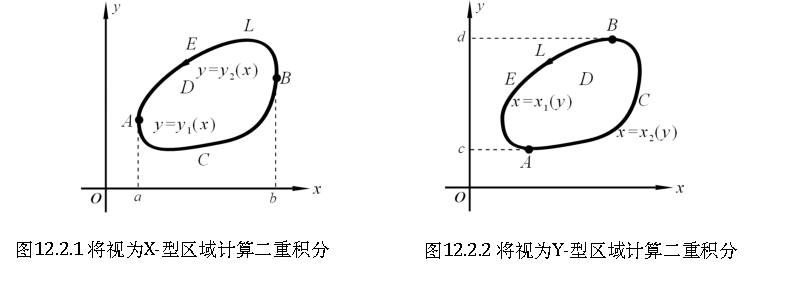
\includegraphics{./images/ch12/xy-Green.pdf}}
\end{center}
事实上,如图12.2.2,区域$D$可以表示为
$$D:y_1\leq y\leq y_2,\;x_1(y)\leq x\leq x_2(y).$$
故
\begin{eqnarray*}
	\mbox{右边}&=&\dint_{y_1}^{y_2}\dint_{x_1(y)}^{x_2(y)}
	Q'_y(x,y)\d x\d y\\
	&=&\dint_{y_1}^{y_2}\left.Q(x,y)\right|_{x_1(y)}^{x_2(y)}\d y\\
	&=&\dint_{y_1}^{y_2}\left[Q(x_2(y),y)-Q(x_1(y),y)\right]\d y
\end{eqnarray*}
又$L=L_1+L_2$,故
\begin{eqnarray*}
	\mbox{左边}&=&\left(\dint_{L_1}+\dint_{L_2}\right)Q(x,y)\d y\\
	&=&\dint_{y_2}^{y_1}Q(x_1(y),y)\d y+\dint_{y_1}^{y_2}Q(x_2(y),y)\d y\\
	&=&\mbox{右边}
\end{eqnarray*}

同理,可以证明:$\ds\oint_LP(x,y)\d x=-\ds\iint_D\df{\p P}{\p y}\d\sigma$。

{\bf 思考:}为什么两个部分存在符号上的差异?({\it 因为曲线靠近$x,y$的部分的方向与两个
坐标轴的相对方向不同!})


{\bf 例:}计算曲线积分$\dint_Lx\d y-y\d x$,其中$L:\df{x^2}{a^2}+\df{y^2}{b^2}=1$
取逆时针方向。

{\bf 提示:}由Green公式
$$\dint_Lx\d y-y\d x=2\iint_D\d\sigma=2\pi ab.$$
事实上,如果直接计算该曲线积分,令$x=a\cos t,y=b\sin t,t\in[0,2\pi]$,则
$$\dint_Lx\d y-y\d x=\dint_0^{2\pi}a\cos t\d(b\sin t)
-b\sin t\d(a\cos t)=ab\dint_0^{2\pi}\d t=2\pi ab.$$

{\bf 注:}该公式可以作为求给定平面区域面积的一种方法,适用于任意边界为分段光滑曲线
的有界闭区域,即
$$S_D=\iint_D\d\sigma=\df12\oint_{\p D}x\d y-y\d x$$

{\bf 关于Green公式的讨论:}
\begin{enumerate}[(1)]
  \setlength{\itemindent}{1cm}
  \item $L$可以包含平行于$x$轴和$y$轴的直线
  \item $D$可以是简单闭区域、单连通域或多连通域
\end{enumerate}

\begin{center}
	\resizebox{!}{10cm}{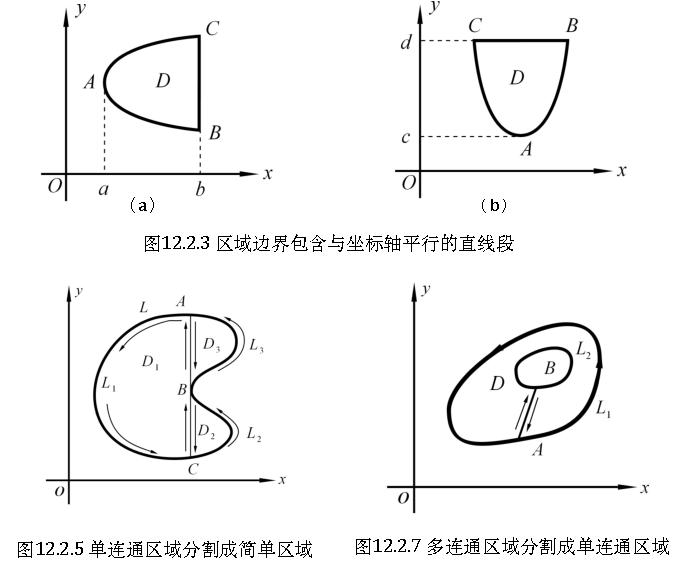
\includegraphics{./images/ch12/d-k.pdf}}
\end{center}

如图12.2.5,
\begin{eqnarray*}
	\iint_D\left(\df{\p Q}{\p x}-\df{\p P}{\p y}\right)\d\sigma&=&
	\left(\iint_{D_1}+\iint_{D_2}+\iint_{D_3}\right)\left(\df{\p Q}{\p x}-\df{\p
	P}{\p y}\right)\d\sigma\\
	&=&\left(\oint_{L_1}+\oint_{L_2}+\oint_{L_3}\right)P\d x+Q\d y\\
	&=&\oint_LP\d x+Q\d y
\end{eqnarray*}

% \begin{shaded}
% 	\centerline{\bf 用差分化方法求曲线积分}
% % 	\begin{tabularx}{\textwidth}{XX}
% % 		\resizebox{!}{6.5cm}{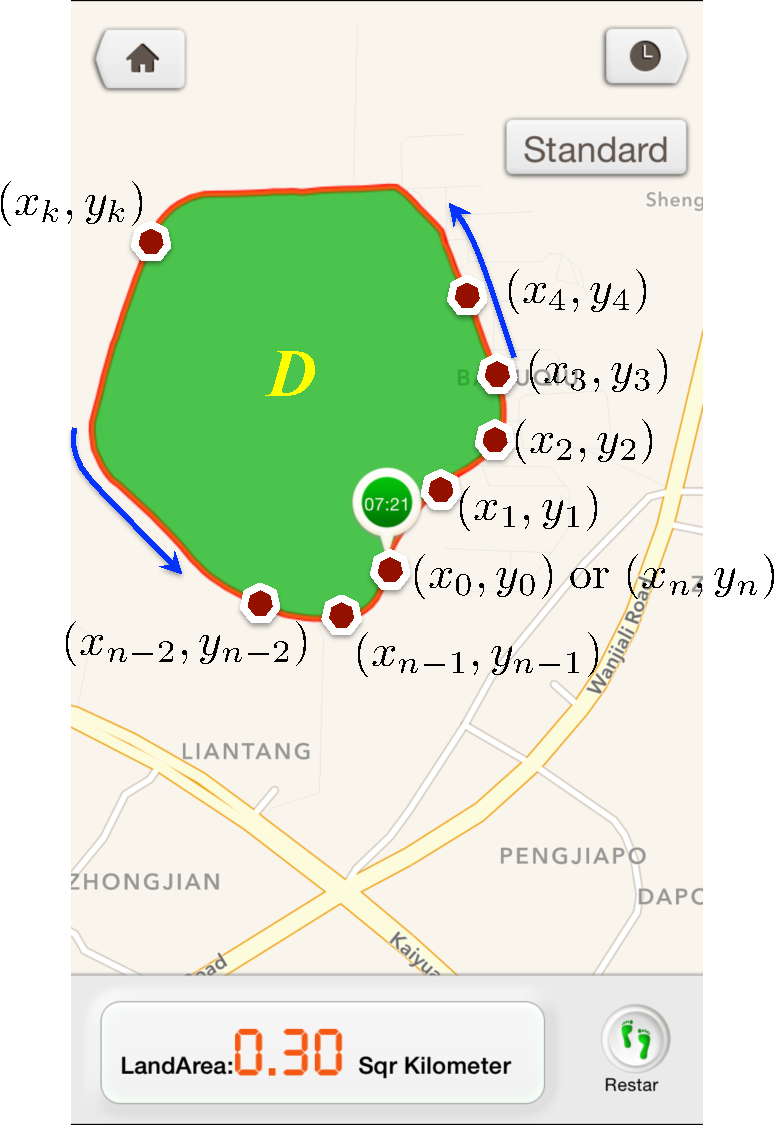
\includegraphics{./images/ch12/YCSam.pdf}}
% % 		&
% % 		$$\ds\iint_D\d\sigma=\df12\ds\oint_Lx\d y-y\d x
% % 		\approx\df12\sum\limits_{k=1}^n$$
% % 		其中
% % 		\begin{itemize}
% % 		  \item $(x_k,y_k)\;(k=0,1,2,\ldots,n)$:GPS采样点 
% % 		  \item $\Delta x_k=x_k-x_{k-1},k=1,2,\ldots,n$ 
% % 		  \item $\Delta y_k=y_k-y_{k-1},\;k=1,2,\ldots,n$
% % 		\end{itemize}
% % 	\end{tabularx}
% % 	\begin{tabular}{cl}
% % 		\resizebox{!}{6.5cm}{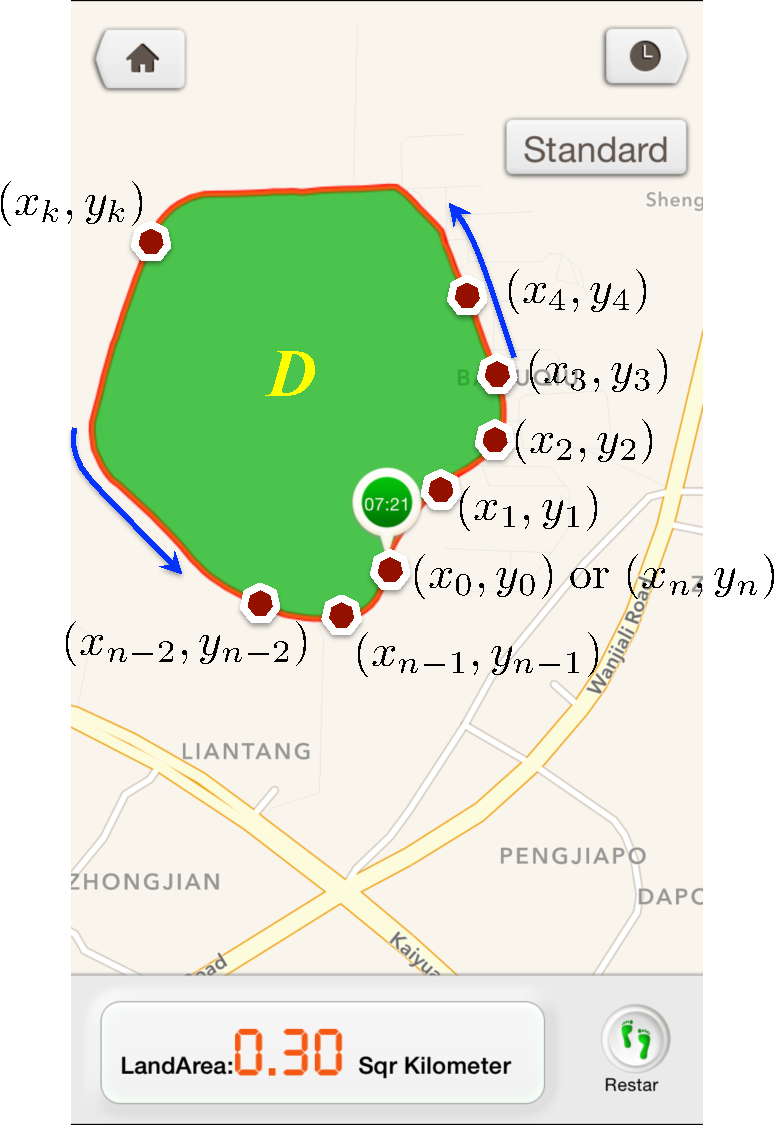
\includegraphics{./images/ch12/YCSam.pdf}}
% % 		&
% % 		$$\ds\iint_D\d\sigma=\df12\ds\oint_Lx\d y-y\d x
% % 		\approx\df12\sum\limits_{k=1}^n$$
% % 		其中
% % 		\begin{itemize}
% % 		  \item $(x_k,y_k)\;(k=0,1,2,\ldots,n)$:GPS采样点
% % 		  \item $\Delta x_k=x_k-x_{k-1},k=1,2,\ldots,n$
% % 		  \item $\Delta y_k=y_k-y_{k-1},\;k=1,2,\ldots,n$
% % 		\end{itemize}
% % 	\end{tabular}
% 	
% % 	$$\ds\iint_D\d\sigma=\df12\ds\oint_Lx\d y-y\d x
% % 	\approx\df12\sum\limits_{k=1}^n$$
% % 	其中
% % 	\begin{itemize}
% % 	  \item $(x_k,y_k)\;(k=0,1,2,\ldots,n)$:GPS采样点
% % 	  \item $\Delta x_k=x_k-x_{k-1},k=1,2,\ldots,n$
% % 	  \item $\Delta y_k=y_k-y_{k-1},\;k=1,2,\ldots,n$
% % 	\end{itemize}
% % 	\begin{center}
% % 		\resizebox{!}{6.5cm}{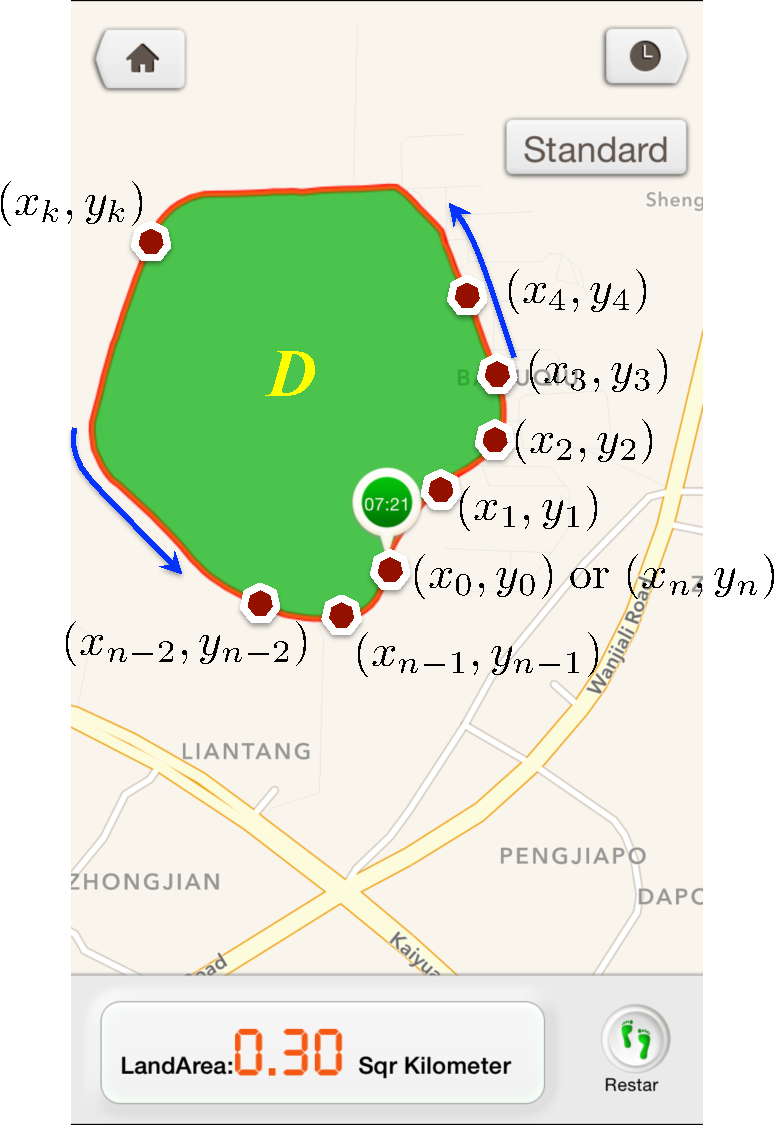
\includegraphics{./images/ch12/YCSam.pdf}}
% % 	\end{center}
% 	
% 	\begin{figure}[htbp]%
% 		\centering
% 		\begin{minipage}[b]{0.4\textwidth}
% 			\centering
% 			\resizebox{!}{7cm}{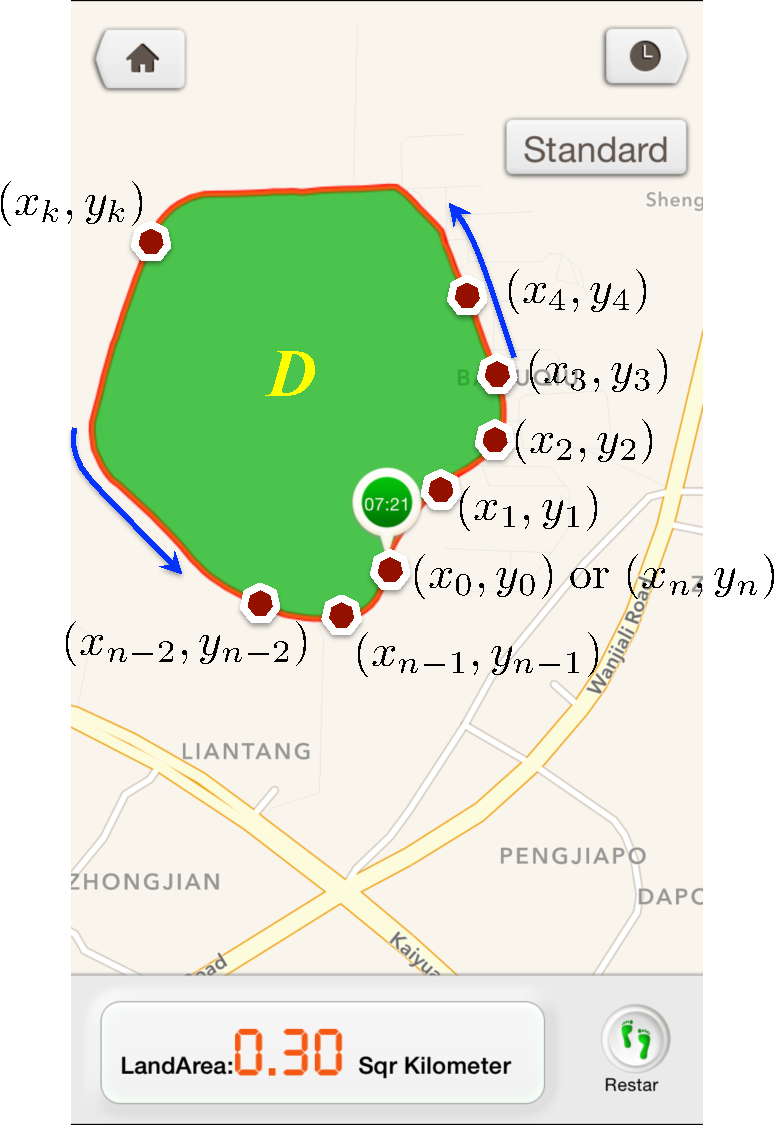
\includegraphics{./images/ch12/YCSam.pdf}}
% 	% 		\caption{清明}
% 		\end{minipage}
% 		\begin{minipage}[b]{0.5\textwidth}
% 			$$\ds\iint_D\d\sigma=\df12\ds\oint_Lx\d y-y\d x
% 			\approx\df12\sum\limits_{k=1}^n$$
% 			其中
% 			\begin{itemize}
% 			  \item $(x_k,y_k)\;(k=0,1,2,\ldots,n)$:GPS采样点
% 			  \item $\Delta x_k=x_k-x_{k-1},k=1,2,\ldots,n$
% 			  \item $\Delta y_k=y_k-y_{k-1},\;k=1,2,\ldots,n$
% 			\end{itemize}
% 		\end{minipage}
% 	\end{figure}
% \end{shaded}

\bigskip

\hrule

\bigskip

\begin{figure}[htbp]%
	\centering
	\begin{minipage}{0.4\textwidth}
		\centering
		\resizebox{!}{7cm}{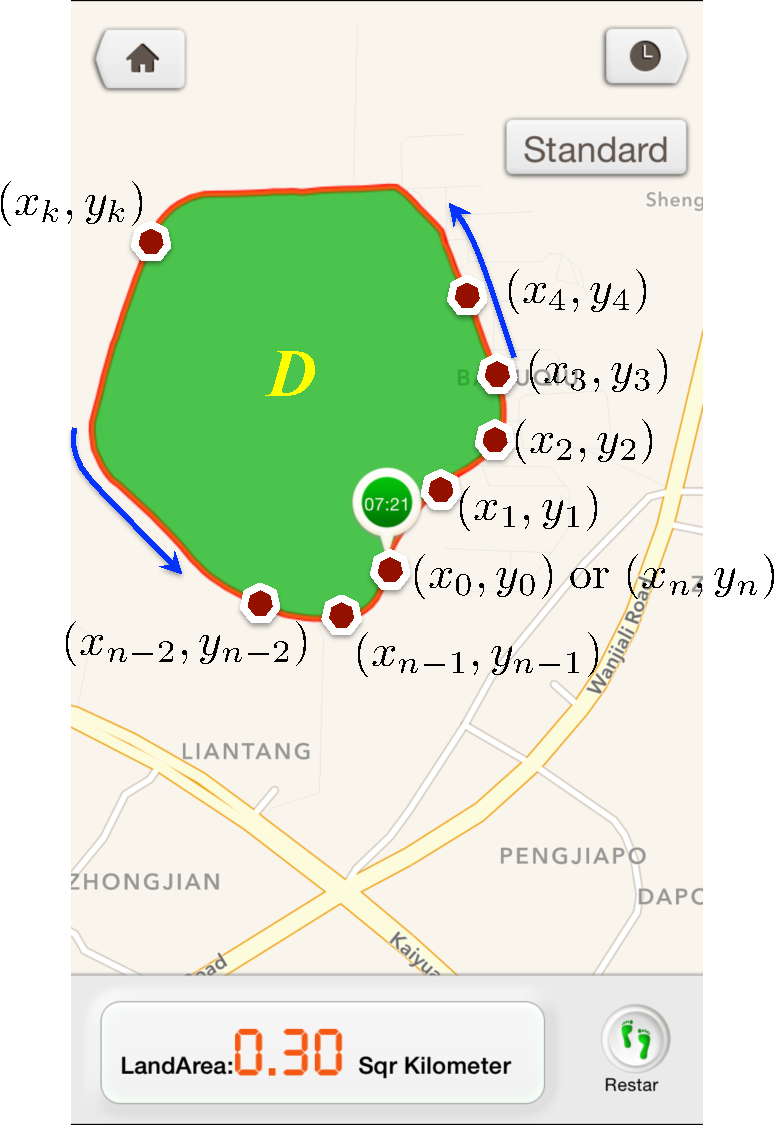
\includegraphics{./images/ch12/YCSam.pdf}}
% 		\caption{清明}
	\end{minipage}
	\begin{minipage}{0.5\textwidth}
		{\bf 用差分化方法求曲线积分}
		\begin{eqnarray*}
			\ds\iint_D\d\sigma&=&\df12\ds\oint_Lx\d y-y\d x\\
			&\approx&\df12\sum\limits_{k=1}^n(x_k\Delta y_k-y_k\Delta x_k)
		\end{eqnarray*}
		其中
		\begin{itemize}
		  \item $(x_k,y_k)\;(k=0,1,2,\ldots,n)$:GPS采样点
		  \item $\Delta x_k=x_k-x_{k-1},k=1,2,\ldots,n$
		  \item $\Delta y_k=y_k-y_{k-1},\;k=1,2,\ldots,n$
		\end{itemize}
	\end{minipage}
\end{figure}

\bigskip

\hrule

\bigskip

{\bf 小结}

\begin{enumerate}[(1)]
  \setlength{\itemindent}{1cm}
  \item Green公式
  	$$\oint_LP\d x+Q\d y=\iint_D\left(
	\df{\p Q}{\p x}-\df{\p P}{\p y}\right)\d\sigma$$
	\begin{itemize}
	  \item 掌握证明的基本思路
	  \item 正确理解定理条件
	\end{itemize}
  \item 利用Green公式求平面区域面积
    $$\ds\iint_D\d\sigma=\df12\ds\oint_Lx\d y-y\d x$$
\end{enumerate}

{\bf 课后作业:}习题12.2:1,3,4

\bigskip

\hrule

\bigskip

{\bf 课后思考:}查阅关于{\it Planimeter(求积仪)}的资料,结合Green公式
解释其工作原理。

\begin{center}
	\resizebox{!}{7cm}{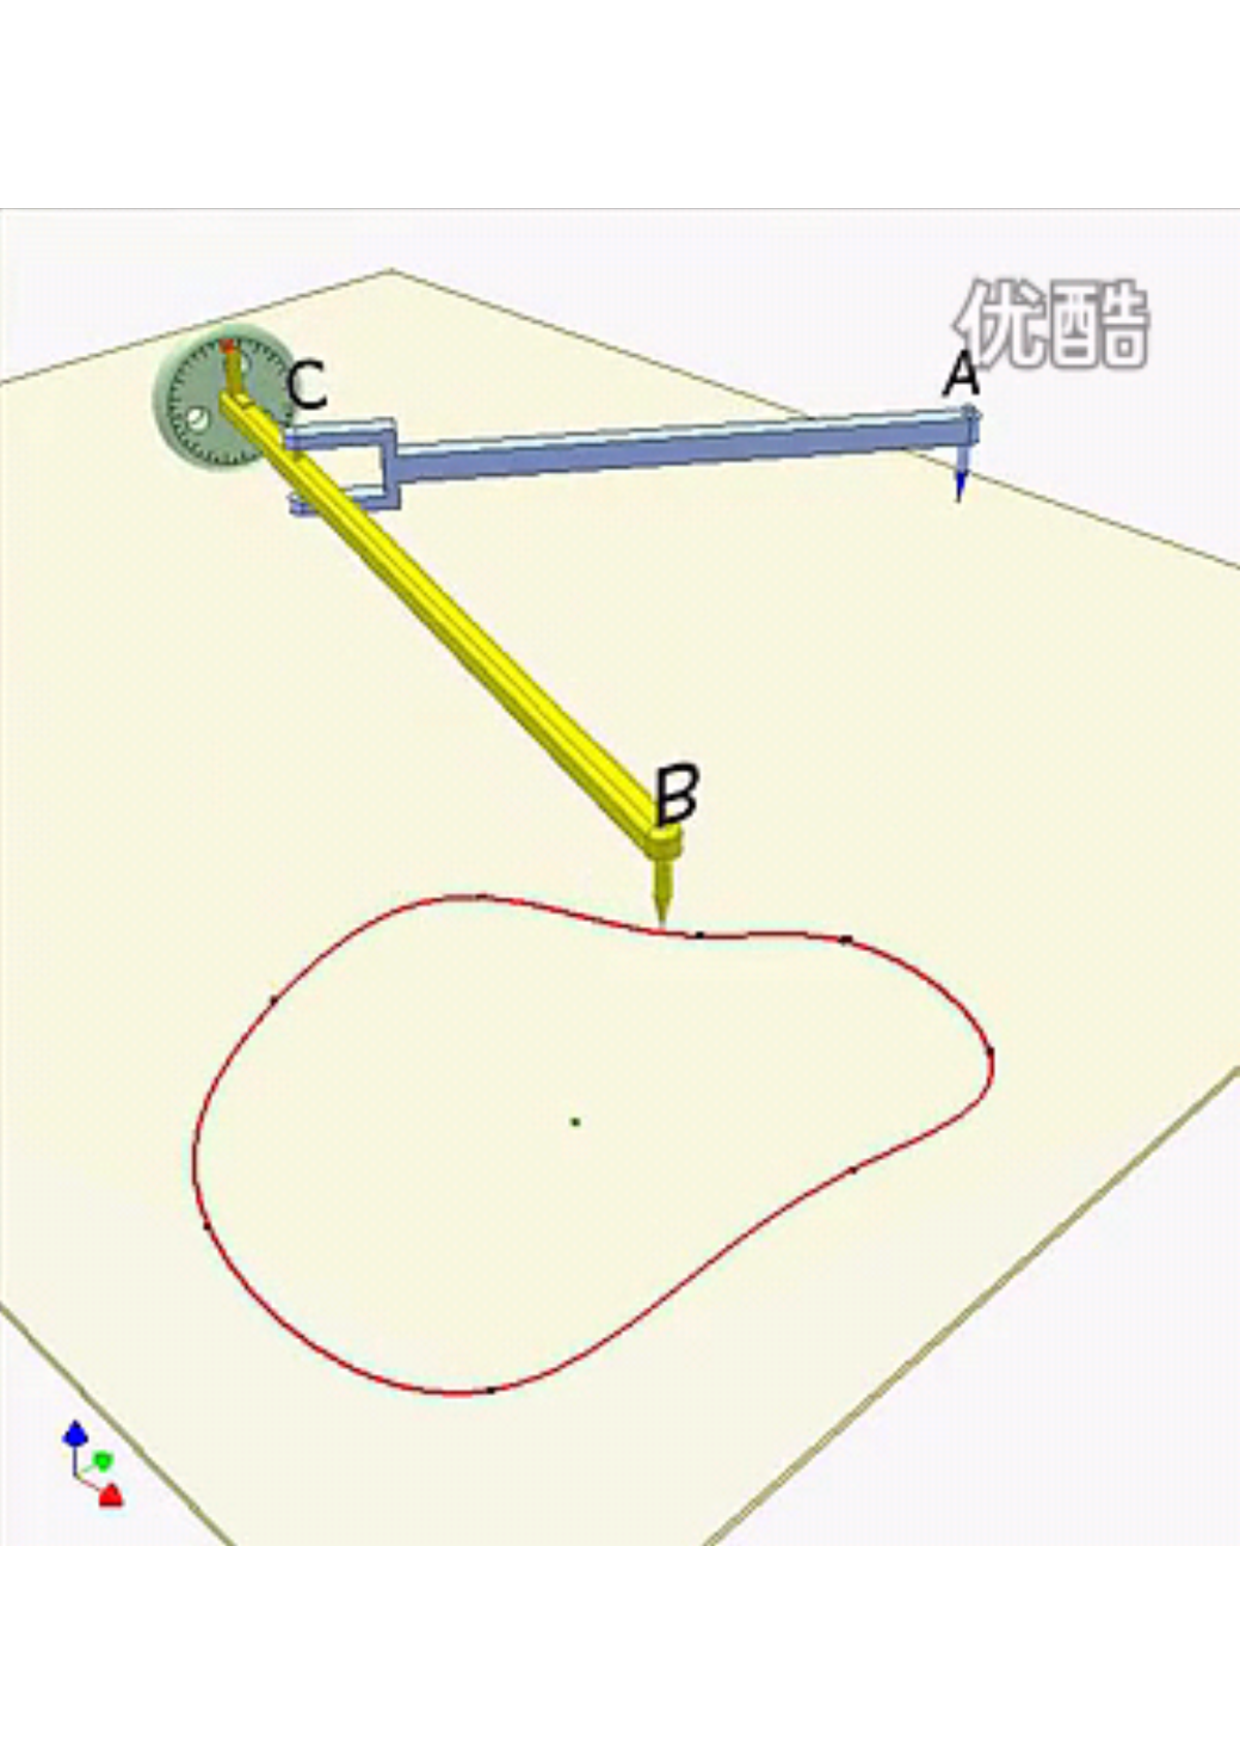
\includegraphics{./images/ch12/planiMeter.pdf}}
	
	(http://v.youku.com/v\_show/id\_XNzIzMDkzMTgw.html?from=s1.8-1-1.2)
\end{center}